\name{DMITRII OKUNEV}


\begin{resume}
\vspace{0.1in}

\iffalse
\vspace{-6.5em}
\flushright
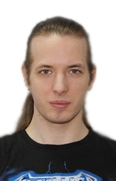
\includegraphics[width=20mm]{photo.jpg}\\
\begin{tabular}{ll}
 {\bf Age} & 30\\
\end{tabular}
\flushleft

\vspace{-5.5em}
\fi

\section{CONTACTS AND SOCIAL PAGES}
\vspace{0.1in} 
\begin{tabular}{ll}
 {\bf E-mail}   & xaionaro@gmail.com (PGP id: 8E30679C)\\
 {\bf GitHub}   & https://github.com/xaionaro\\
 {\bf LinkedIn} & https://www.linkedin.com/in/dmitry-okunev/\\
\end{tabular}

\section{EDUCATION}
\vspace{0.1in} 
\begin{tabular}{ll}
 {\bf 2013-2017} & Postgraduate education (incomplete PhD), thermal physics, NRNU MEPhI, Moscow, Russia\\
 {\bf 2006-2013} & Kinetic physics specialist, engineer-physicist, NRNU MEPhI, Moscow, Russia\\
\end{tabular}

\section{EMPLOYMENT}
\vspace{0.1in} 
\begin{tabular}{ll}
    {\bf 2019-now}  & Production Engineer, Facebook\\
    {\bf 2018-2019} & Senior backend engineer (Golang), Wisebits\\
    {\bf 2017-2018} & DevOps, JSC "TelemedHelp"\\
    {\bf 2012-2018} & Head of a system administrating department (head of UNIX-tech\\
                    & department), NRNU MEPhI\\
    {\bf 2011-2012} & System administrator team lead, department of Telecommunications,\\
                    & NRNU MEPhI\\
    {\bf 2009-2011} & Network engineer and system administrator, department of \\
                    & Telecommunications, NRNU MEPhI\\
    {\bf 2007-2009} & System administrator (specialist in telematic services), JSC "Rosnet"\\
\end{tabular}

\section{MAIN ACTIVITIES}
\vspace{0.1in} 
\begin{tabular}{lrl}
    {\bf 2019-now}  & Facebook        & Developing the remote attestation infrastructure.\\
                    &                 & The main expertise area: BIOS firmware remote attestation.\\
                    &                 & In particular, it includes designing and development of testing,\\
                    &                 & diagnostics and remediation distributed automation, validation\\
                    &                 & of security designs, negotiations with vendors, people management\\
                    &                 & and other.\\
    {\bf 2018-2019} & Wisebits        & Developing highload solutions (80KQPS). Stabilized the product;\\
                    &                 & implemented high-performance metrics; made lot of fixes, monitoring,\\
                    &                 & new features and so on.\\
    {\bf 2017-2018} & JSC TelemedHelp & Created HA/LB infrastructure with CI/CD.\\
    {\bf 2009-2018} & NRNU MEPhI      & Created: an UNIX tech department itself, VoIP, HPC center\\
                    &                 & (with 4 HPC-clusters), VPN-services, LXC-based HA Linux hosting,\\
                    &                 & ftp.ru.debian.org and so on.\\
                    &                 & While managing the department I've automated related University\\
                    &                 & processes.\\
    {\bf 2007-2009} & JSC Rosnet      & Adminitrating mail server (including mail of a Russian Ministry),\\
                    &                 & billing, web servers etc; created a mail anti-DDoS protection.\\
    {\bf 2006-2007} & UltaNetwork     & Created an unofficial campus network.\\
    {\bf 2005-2007} & RootNet/IrcCity & Developed different utilities (anti-DDoS, different services).\\
\end{tabular}
\end{resume}
